% !TEX root = ../main.tex
\chapter{Results}
\label{ch:results}

When streaming from the sample stream, from which the sample dataset was collected,
the topic distribution does not approach that of the sample dataset.
While the topic distribution on the training dataset is close to equally distributed as seen in~\ref{fig:sample_topic_distribution},
the same cannot be said for the topic distribution on the same stream on September $27^{th}$ 2017, more than two months later,
as seen in~\ref{fig:sample_topic_distribtion_new}.

\begin{figure}
    \centering
    \caption{Topic distribution of new data, with the LDA model trained on the sample dataset}
    \label{fig:sample_topic_distribtion_new}
    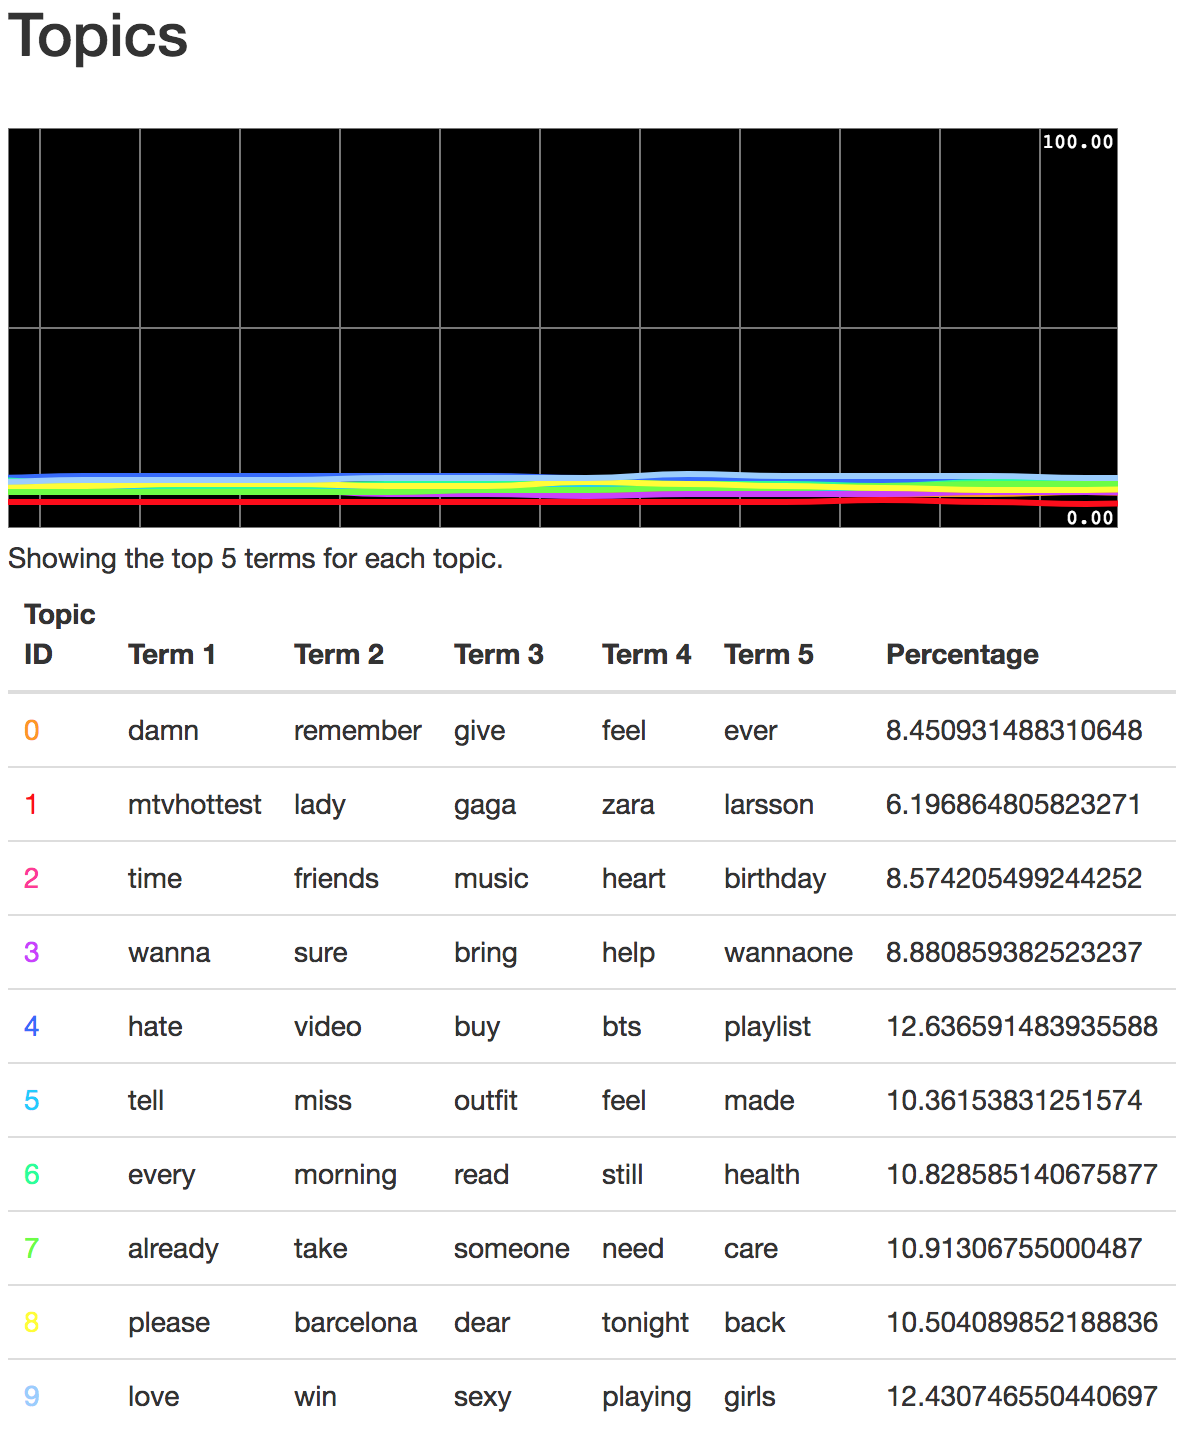
\includegraphics[width=\textwidth]{../images/dashboard_topics_sample.png}
\end{figure}

This time, topics with top terms that indicate some event, like "mtvhottest", are lower in prevalence,
in favor of topics with more general terms.\\
This indicates that while the dashboard can reliably show changes in what users are talking about on Twitter,
as demonstrated in~\ref{sec:testing},
it might not be able to accurately model new, emerging topics.
\\
For this reason, it also does not make sense to compare the sentiment by topic distributions,
since the meaning of topics changed.
\par
The same comparison was however made for sentiment analysis, comparing the sentiment distribution in the sample dataset, seen in~\ref{fig:sample_sentiment},
to the sentiment distribution observed through the dashboard on the 27$^th$ of September 2017, seen in~\ref{fig:sample_sentiment_distribtion_new}.

\begin{figure}
    \centering
    \caption{Sentiment distribution of new data, with the naive bayes model trained on the sanders dataset}
    \label{fig:sample_sentiment_distribtion_new}
    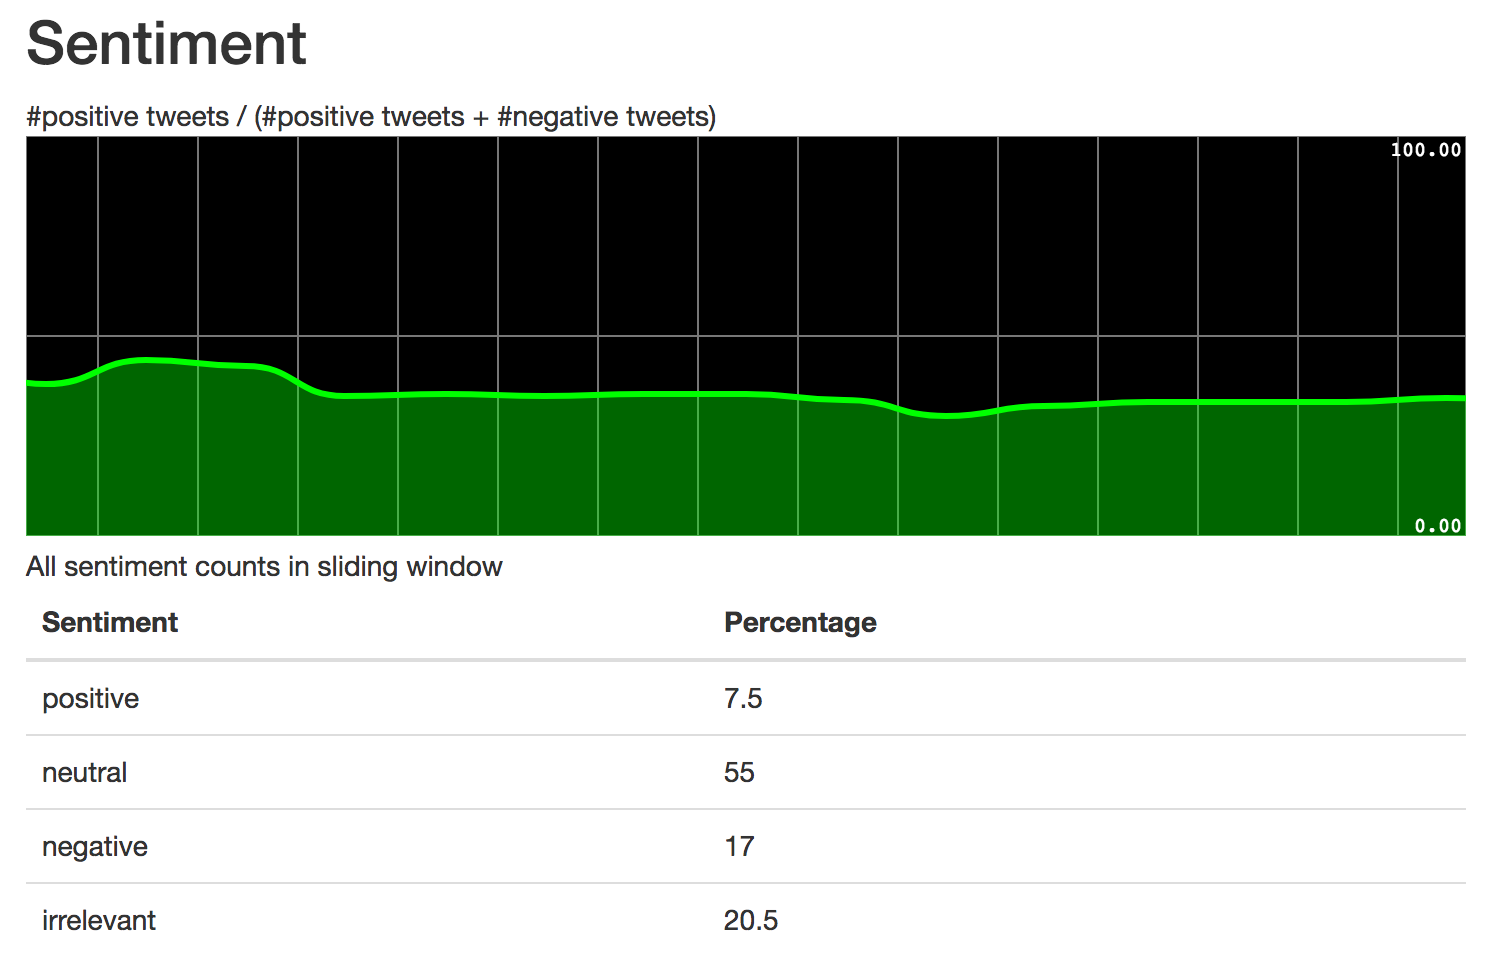
\includegraphics[width=\textwidth]{../images/dashboard_sentiment_sample.png}
\end{figure}

This comparison shows that the sentiment on the stream remained on a similar level than in the sample dataset,
and did not change as much as the topics did, indicating that while the topics twitter users post statuses about change,
the overall, average sentiment, remains relatively constant.

\par
In spite of some shortcomings, the dashboard therefore still provides interesting insights and monitoring capabilities.
\\
It can, for example, be used to track a companies Twitter feed during a critical event, using the user stream.
This would provide an objective indication of the events impact on customer sentiment,
and enable the company to react in real time without having to base a decision on few, manually observed interactions.
\\
It can also be used to monitor a stream for sudden changes in topic,
indicating the occurrence of an event that might be of interest for the monitoring entity.